% !TeX program = pdfLaTeX
\documentclass[12pt]{article}
\usepackage{amsmath}
\usepackage{graphicx,psfrag,epsf}
\usepackage{enumerate}
\usepackage{natbib}
\usepackage{textcomp}
\usepackage[hyphens]{url} % not crucial - just used below for the URL
\usepackage{hyperref}
\providecommand{\tightlist}{%
  \setlength{\itemsep}{0pt}\setlength{\parskip}{0pt}}

%\pdfminorversion=4
% NOTE: To produce blinded version, replace "0" with "1" below.
\newcommand{\blind}{0}

% DON'T change margins - should be 1 inch all around.
\addtolength{\oddsidemargin}{-.5in}%
\addtolength{\evensidemargin}{-.5in}%
\addtolength{\textwidth}{1in}%
\addtolength{\textheight}{1.3in}%
\addtolength{\topmargin}{-.8in}%

%% load any required packages here


\usepackage{color}
\usepackage{fancyvrb}
\newcommand{\VerbBar}{|}
\newcommand{\VERB}{\Verb[commandchars=\\\{\}]}
\DefineVerbatimEnvironment{Highlighting}{Verbatim}{commandchars=\\\{\}}
% Add ',fontsize=\small' for more characters per line
\usepackage{framed}
\definecolor{shadecolor}{RGB}{248,248,248}
\newenvironment{Shaded}{\begin{snugshade}}{\end{snugshade}}
\newcommand{\AlertTok}[1]{\textcolor[rgb]{0.94,0.16,0.16}{#1}}
\newcommand{\AnnotationTok}[1]{\textcolor[rgb]{0.56,0.35,0.01}{\textbf{\textit{#1}}}}
\newcommand{\AttributeTok}[1]{\textcolor[rgb]{0.77,0.63,0.00}{#1}}
\newcommand{\BaseNTok}[1]{\textcolor[rgb]{0.00,0.00,0.81}{#1}}
\newcommand{\BuiltInTok}[1]{#1}
\newcommand{\CharTok}[1]{\textcolor[rgb]{0.31,0.60,0.02}{#1}}
\newcommand{\CommentTok}[1]{\textcolor[rgb]{0.56,0.35,0.01}{\textit{#1}}}
\newcommand{\CommentVarTok}[1]{\textcolor[rgb]{0.56,0.35,0.01}{\textbf{\textit{#1}}}}
\newcommand{\ConstantTok}[1]{\textcolor[rgb]{0.00,0.00,0.00}{#1}}
\newcommand{\ControlFlowTok}[1]{\textcolor[rgb]{0.13,0.29,0.53}{\textbf{#1}}}
\newcommand{\DataTypeTok}[1]{\textcolor[rgb]{0.13,0.29,0.53}{#1}}
\newcommand{\DecValTok}[1]{\textcolor[rgb]{0.00,0.00,0.81}{#1}}
\newcommand{\DocumentationTok}[1]{\textcolor[rgb]{0.56,0.35,0.01}{\textbf{\textit{#1}}}}
\newcommand{\ErrorTok}[1]{\textcolor[rgb]{0.64,0.00,0.00}{\textbf{#1}}}
\newcommand{\ExtensionTok}[1]{#1}
\newcommand{\FloatTok}[1]{\textcolor[rgb]{0.00,0.00,0.81}{#1}}
\newcommand{\FunctionTok}[1]{\textcolor[rgb]{0.00,0.00,0.00}{#1}}
\newcommand{\ImportTok}[1]{#1}
\newcommand{\InformationTok}[1]{\textcolor[rgb]{0.56,0.35,0.01}{\textbf{\textit{#1}}}}
\newcommand{\KeywordTok}[1]{\textcolor[rgb]{0.13,0.29,0.53}{\textbf{#1}}}
\newcommand{\NormalTok}[1]{#1}
\newcommand{\OperatorTok}[1]{\textcolor[rgb]{0.81,0.36,0.00}{\textbf{#1}}}
\newcommand{\OtherTok}[1]{\textcolor[rgb]{0.56,0.35,0.01}{#1}}
\newcommand{\PreprocessorTok}[1]{\textcolor[rgb]{0.56,0.35,0.01}{\textit{#1}}}
\newcommand{\RegionMarkerTok}[1]{#1}
\newcommand{\SpecialCharTok}[1]{\textcolor[rgb]{0.00,0.00,0.00}{#1}}
\newcommand{\SpecialStringTok}[1]{\textcolor[rgb]{0.31,0.60,0.02}{#1}}
\newcommand{\StringTok}[1]{\textcolor[rgb]{0.31,0.60,0.02}{#1}}
\newcommand{\VariableTok}[1]{\textcolor[rgb]{0.00,0.00,0.00}{#1}}
\newcommand{\VerbatimStringTok}[1]{\textcolor[rgb]{0.31,0.60,0.02}{#1}}
\newcommand{\WarningTok}[1]{\textcolor[rgb]{0.56,0.35,0.01}{\textbf{\textit{#1}}}}


\usepackage{float} \floatplacement{figure}{H}
\usepackage{booktabs}
\usepackage{longtable}
\usepackage{array}
\usepackage{multirow}
\usepackage{wrapfig}
\usepackage{float}
\usepackage{colortbl}
\usepackage{pdflscape}
\usepackage{tabu}
\usepackage{threeparttable}
\usepackage{threeparttablex}
\usepackage[normalem]{ulem}
\usepackage{makecell}
\usepackage{xcolor}

\begin{document}


\def\spacingset#1{\renewcommand{\baselinestretch}%
{#1}\small\normalsize} \spacingset{1}


%%%%%%%%%%%%%%%%%%%%%%%%%%%%%%%%%%%%%%%%%%%%%%%%%%%%%%%%%%%%%%%%%%%%%%%%%%%%%%

\if0\blind
{
  \title{\bf MATH2269 Semester 2 2020 - Final Project}

  \author{
        Sam Holt, Phil Steinke, Elleni Toumpas \\
    RMIT\\
      }
  \maketitle
} \fi

\if1\blind
{
  \bigskip
  \bigskip
  \bigskip
  \begin{center}
    {\LARGE\bf MATH2269 Semester 2 2020 - Final Project}
  \end{center}
  \medskip
} \fi

\bigskip
\begin{abstract}
Insert Abstract
\end{abstract}

\noindent%
{\it Keywords:} JAGS, multiple linear regression analysis, prediction
\vfill

\newpage
\spacingset{1.45} % DON'T change the spacing!

\hypertarget{introduction}{%
\section{Introduction}\label{introduction}}

\hypertarget{analysis}{%
\section{Analysis}\label{analysis}}

\hypertarget{a-descriptive-look}{%
\subsection{A descriptive look}\label{a-descriptive-look}}

\hypertarget{dimensions}{%
\subsubsection{Dimensions}\label{dimensions}}

\begin{longtable}[]{@{}rr@{}}
\caption{Dimenions}\tabularnewline
\toprule
columns & rows\tabularnewline
\midrule
\endfirsthead
\toprule
columns & rows\tabularnewline
\midrule
\endhead
28 & 25626\tabularnewline
\bottomrule
\end{longtable}

\begin{landscape}\begin{table}

\caption{\label{tab:unnamed-chunk-2}Inspecting the first six rows of the data.}
\centering
\fontsize{6}{8}\selectfont
\begin{tabu} to \linewidth {>{\raggedleft}X>{\raggedleft}X>{\raggedleft}X>{\raggedleft}X>{\raggedleft}X>{\raggedleft}X}
\hline
\rotatebox{90}{id} & \rotatebox{90}{rainfall\_mm} & \rotatebox{90}{rf\_cum\_2\_day} & \rotatebox{90}{rf\_cum\_3\_day} & \rotatebox{90}{rf\_cum\_4\_day} & \rotatebox{90}{rf\_cum\_5\_day}\\
\hline
1 & 0 & 0 & 0 & 0 & 0.2\\
\hline
2 & 0 & 0 & 0 & 0 & 0.2\\
\hline
3 & 0 & 0 & 0 & 0 & 0.2\\
\hline
4 & 0 & 0 & 0 & 0 & 0.2\\
\hline
5 & 0 & 0 & 0 & 0 & 0.2\\
\hline
\end{tabu}
\end{table}
\end{landscape}

\begin{landscape}\begin{table}

\caption{\label{tab:unnamed-chunk-2}Inspecting the first six rows of the data.}
\centering
\fontsize{6}{8}\selectfont
\begin{tabu} to \linewidth {>{\raggedleft}X>{\raggedleft}X>{\raggedright}X>{\raggedright}X>{\raggedright}X}
\hline
\rotatebox{90}{rf\_cum\_6\_day} & \rotatebox{90}{rf\_cum\_7\_day} & \rotatebox{90}{date\_day} & \rotatebox{90}{date\_local\_time} & \rotatebox{90}{site}\\
\hline
1 & 25.6 & 2016-01-01 & 2016-01-01 00:00:00 & Brooklyn\\
\hline
1 & 25.6 & 2016-01-01 & 2016-01-01 01:00:00 & Brooklyn\\
\hline
1 & 25.6 & 2016-01-01 & 2016-01-01 02:00:00 & Brooklyn\\
\hline
1 & 25.6 & 2016-01-01 & 2016-01-01 03:00:00 & Brooklyn\\
\hline
1 & 25.6 & 2016-01-01 & 2016-01-01 04:00:00 & Brooklyn\\
\hline
\end{tabu}
\end{table}
\end{landscape}

\begin{landscape}\begin{table}

\caption{\label{tab:unnamed-chunk-2}Inspecting the first six rows of the data.}
\centering
\fontsize{6}{8}\selectfont
\begin{tabu} to \linewidth {>{\raggedleft}X>{\raggedleft}X>{\raggedleft}X>{\raggedleft}X>{\raggedleft}X>{\raggedright}X>{\raggedleft}X>{\raggedright}X}
\hline
\rotatebox{90}{temperature} & \rotatebox{90}{pm10} & \rotatebox{90}{pm10a} & \rotatebox{90}{wd} & \rotatebox{90}{ws} & \rotatebox{90}{dow} & \rotatebox{90}{hour} & \rotatebox{90}{winddire}\\
\hline
23.9 & 30.5 & 30.5 & 263 & 1.6 & Friday & 0 & W\\
\hline
23.5 & 25.8 & 25.8 & 282 & 1.3 & Friday & 1 & WNW\\
\hline
23.1 & 22.2 & 22.2 & 288 & 1.1 & Friday & 2 & WNW\\
\hline
22.1 & 23.2 & 23.2 & 340 & 0.9 & Friday & 3 & NNW\\
\hline
21.4 & 24.3 & 24.3 & 328 & 0.8 & Friday & 4 & NNW\\
\hline
\end{tabu}
\end{table}
\end{landscape}

\begin{landscape}\begin{table}

\caption{\label{tab:unnamed-chunk-2}Inspecting the first six rows of the data.}
\centering
\fontsize{6}{8}\selectfont
\begin{tabu} to \linewidth {>{\raggedleft}X>{\raggedright}X>{\raggedleft}X>{\raggedright}X>{\raggedright}X>{\raggedright}X>{\raggedright}X>{\raggedright}X>{\raggedright}X}
\hline
\rotatebox{90}{years} & \rotatebox{90}{yn80} & \rotatebox{90}{roll\_temp} & \rotatebox{90}{yn50} & \rotatebox{90}{north} & \rotatebox{90}{north1} & \rotatebox{90}{yn60} & \rotatebox{90}{weekdays} & \rotatebox{90}{mornings}\\
\hline
2016 & FALSE & NA & FALSE & FALSE & FALSE & FALSE & TRUE & FALSE\\
\hline
2016 & FALSE & NA & FALSE & TRUE & FALSE & FALSE & TRUE & \vphantom{1} FALSE\\
\hline
2016 & FALSE & NA & FALSE & TRUE & FALSE & FALSE & TRUE & FALSE\\
\hline
2016 & FALSE & NA & FALSE & TRUE & TRUE & FALSE & TRUE & \vphantom{1} FALSE\\
\hline
2016 & FALSE & NA & FALSE & TRUE & TRUE & FALSE & TRUE & FALSE\\
\hline
\end{tabu}
\end{table}
\end{landscape}

\hypertarget{datatypes}{%
\subsubsection{Datatypes}\label{datatypes}}

The datatypes for each variable can be found below (after variable
datatypes were set on import). Numerical variables that are actually
binary values or an identifier were transformed to a factor.

\begin{table}

\caption{\label{tab:unnamed-chunk-3}Data types}
\centering
\begin{tabu} to \linewidth {>{\raggedright}X>{\raggedright}X}
\hline
  & class\\
\hline
id & numeric\\
\hline
rainfall\_mm & numeric\\
\hline
rf\_cum\_2\_day & numeric\\
\hline
rf\_cum\_3\_day & numeric\\
\hline
rf\_cum\_4\_day & numeric\\
\hline
rf\_cum\_5\_day & numeric\\
\hline
rf\_cum\_6\_day & numeric\\
\hline
rf\_cum\_7\_day & numeric\\
\hline
date\_day & Date\\
\hline
date\_local\_time & POSIXct POSIXt\\
\hline
site & character\\
\hline
temperature & numeric\\
\hline
pm10 & numeric\\
\hline
pm10a & numeric\\
\hline
wd & numeric\\
\hline
ws & numeric\\
\hline
dow & character\\
\hline
hour & numeric\\
\hline
winddire & character\\
\hline
years & numeric\\
\hline
yn80 & logical\\
\hline
roll\_temp & numeric\\
\hline
yn50 & logical\\
\hline
north & logical\\
\hline
north1 & logical\\
\hline
yn60 & logical\\
\hline
weekdays & logical\\
\hline
mornings & logical\\
\hline
\end{tabu}
\end{table}

\hypertarget{data-preprocessing}{%
\subsubsection{Data Preprocessing}\label{data-preprocessing}}

\hypertarget{removing-unique-identifier}{%
\paragraph{Removing unique
identifier}\label{removing-unique-identifier}}

\begin{table}

\caption{\label{tab:unnamed-chunk-4}The count of id variable filtered to show only values that are not unique.}
\centering
\begin{tabu} to \linewidth {>{\raggedleft}X>{\raggedleft}X}
\hline
id & count\\


\hline
\end{tabu}
\end{table}

As confirmed above, the \textbf{id} is a unique identifier, and it is
therefore removed from the dataset.

\hypertarget{target-variable-frequency}{%
\paragraph{Target variable frequency}\label{target-variable-frequency}}

Before moving on to the outlier, impossible value and missing values
check phases, it is important to get an understanding of the frequency
of each level in the target level. This will assist when deciding on the
best method for fixing possible issues in the following phases. If one
of the target levels are only represented by a small number of records
then simply removing the records that fail any of the further checks
will be ill-advised.

\begin{table}

\caption{\label{tab:unnamed-chunk-6}The frequency of different levels in the target variable.}
\centering
\begin{tabu} to \linewidth {>{\raggedright}X>{\raggedleft}X}
\hline
yn80 & count\\
\hline
FALSE & 24988\\
\hline
TRUE & 638\\
\hline
\end{tabu}
\end{table}

We can see from the frequency of the target variables that there is a
severely imbalanced dataset. If the decision had to be made on how to
resolve issues in records containing a positive target class, it is
advisable not to remove these records.

\hypertarget{outliers}{%
\paragraph{Outliers}\label{outliers}}

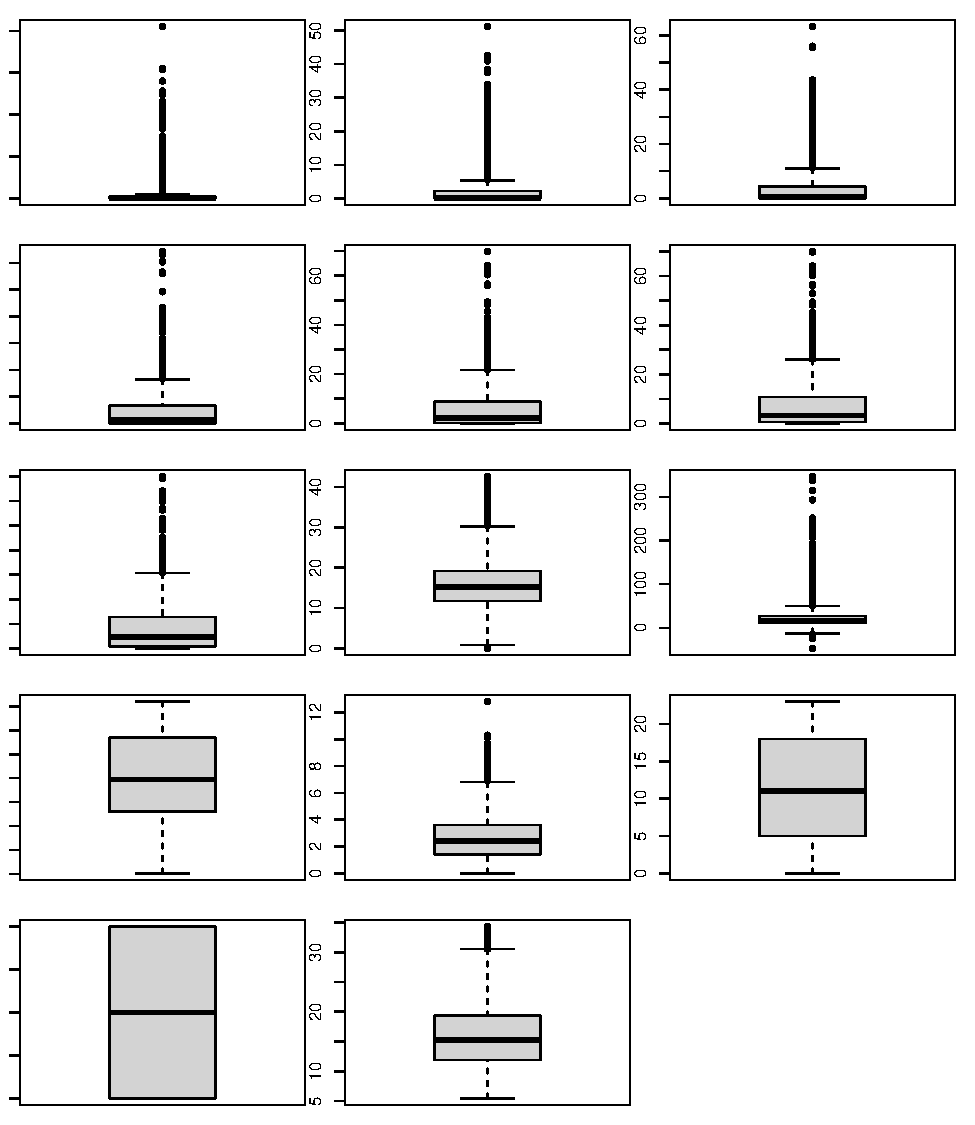
\includegraphics{MATH2269_final_project_files/figure-latex/unnamed-chunk-8-1.pdf}

\hypertarget{impossible-values}{%
\paragraph{Impossible values}\label{impossible-values}}

For the numerical values in the dataset an impossible value check is
performed.

\begin{table}

\caption{\label{tab:unnamed-chunk-9}The number of rows with impossible values.}
\centering
\begin{tabu} to \linewidth {>{\raggedright}X>{\raggedleft}X}
\hline
column & nrows\\
\hline
rainfall\_mm & 0\\
\hline
rf\_cum\_2\_day & 0\\
\hline
rf\_cum\_3\_day & 0\\
\hline
rf\_cum\_4\_day & 0\\
\hline
rf\_cum\_5\_day & 0\\
\hline
rf\_cum\_6\_day & 0\\
\hline
rf\_cum\_7\_day & 0\\
\hline
rf\_cum\_5\_day & 0\\
\hline
date\_day & 0\\
\hline
temperature & 0\\
\hline
pm10 & 118\\
\hline
pm10a & 118\\
\hline
wd & 0\\
\hline
ws & 0\\
\hline
hour & 0\\
\hline
years & 0\\
\hline
roll\_temp & 0\\
\hline
\end{tabu}
\end{table}

\hypertarget{missing-values}{%
\subsubsection{Missing values}\label{missing-values}}

Checking the missing values we can see that there are 23 rolling
temperate missing records.

\begin{table}

\caption{\label{tab:unnamed-chunk-10}Count of missing values by variable}
\centering
\begin{tabu} to \linewidth {>{\raggedright}X>{\raggedleft}X}
\hline
  & Number missing values\\
\hline
rainfall\_mm & 0\\
\hline
rf\_cum\_2\_day & 0\\
\hline
rf\_cum\_3\_day & 0\\
\hline
rf\_cum\_4\_day & 0\\
\hline
rf\_cum\_5\_day & 0\\
\hline
rf\_cum\_6\_day & 0\\
\hline
rf\_cum\_7\_day & 0\\
\hline
date\_day & 0\\
\hline
date\_local\_time & 0\\
\hline
site & 0\\
\hline
temperature & 0\\
\hline
pm10 & 0\\
\hline
pm10a & 0\\
\hline
wd & 0\\
\hline
ws & 0\\
\hline
dow & 0\\
\hline
hour & 0\\
\hline
winddire & 0\\
\hline
years & 0\\
\hline
yn80 & 0\\
\hline
roll\_temp & 23\\
\hline
yn50 & 0\\
\hline
north & 0\\
\hline
north1 & 0\\
\hline
yn60 & 0\\
\hline
weekdays & 0\\
\hline
mornings & 0\\
\hline
\end{tabu}
\end{table}

Inspecing the missing records, we can see that all missing values occur
in the end part of the dataset with no records including a positive
target class.

\begin{Shaded}
\begin{Highlighting}[]
\NormalTok{data_cleaned }\OperatorTok\StringTok{ }
\StringTok{  }\KeywordTok{filter}\NormalTok{(}\KeywordTok{is.na}\NormalTok{(roll_temp)) }\OperatorTok\StringTok{ }
\StringTok{  }\KeywordTok{select}\NormalTok{(date_day, date_local_time, roll_temp, yn80) }\OperatorTok\StringTok{ }
\StringTok{  }\KeywordTok{format_table}\NormalTok{(}\DataTypeTok{p_caption =} \StringTok{"Missing roll temperate values"}\NormalTok{)}
\end{Highlighting}
\end{Shaded}

\begin{table}

\caption{\label{tab:unnamed-chunk-11}Missing roll temperate values}
\centering
\begin{tabu} to \linewidth {>{\raggedright}X>{\raggedright}X>{\raggedleft}X>{\raggedright}X}
\hline
date\_day & date\_local\_time & roll\_temp & yn80\\
\hline
2016-01-01 & 2016-01-01 00:00:00 & NA & FALSE\\
\hline
2016-01-01 & 2016-01-01 01:00:00 & NA & FALSE\\
\hline
2016-01-01 & 2016-01-01 02:00:00 & NA & FALSE\\
\hline
2016-01-01 & 2016-01-01 03:00:00 & NA & FALSE\\
\hline
2016-01-01 & 2016-01-01 04:00:00 & NA & FALSE\\
\hline
2016-01-01 & 2016-01-01 05:00:00 & NA & FALSE\\
\hline
2016-01-01 & 2016-01-01 06:00:00 & NA & FALSE\\
\hline
2016-01-01 & 2016-01-01 07:00:00 & NA & FALSE\\
\hline
2016-01-01 & 2016-01-01 08:00:00 & NA & FALSE\\
\hline
2016-01-01 & 2016-01-01 09:00:00 & NA & FALSE\\
\hline
2016-01-01 & 2016-01-01 10:00:00 & NA & FALSE\\
\hline
2018-12-31 & 2018-12-31 12:00:00 & NA & FALSE\\
\hline
2018-12-31 & 2018-12-31 13:00:00 & NA & FALSE\\
\hline
2018-12-31 & 2018-12-31 14:00:00 & NA & FALSE\\
\hline
2018-12-31 & 2018-12-31 15:00:00 & NA & FALSE\\
\hline
2018-12-31 & 2018-12-31 16:00:00 & NA & FALSE\\
\hline
2018-12-31 & 2018-12-31 17:00:00 & NA & FALSE\\
\hline
2018-12-31 & 2018-12-31 18:00:00 & NA & FALSE\\
\hline
2018-12-31 & 2018-12-31 19:00:00 & NA & FALSE\\
\hline
2018-12-31 & 2018-12-31 20:00:00 & NA & FALSE\\
\hline
2018-12-31 & 2018-12-31 21:00:00 & NA & FALSE\\
\hline
2018-12-31 & 2018-12-31 22:00:00 & NA & FALSE\\
\hline
2018-12-31 & 2018-12-31 23:00:00 & NA & FALSE\\
\hline
\end{tabu}
\end{table}

It is therefore sufficient to simply remove these records from the
dataset.

\begin{Shaded}
\begin{Highlighting}[]
\CommentTok{#### INSERT SAM'S CODE TO REMOVE MISSING VALUES}
\end{Highlighting}
\end{Shaded}

\hypertarget{feature-engineering}{%
\paragraph{Feature engineering}\label{feature-engineering}}

\begin{Shaded}
\begin{Highlighting}[]
\CommentTok{#### Do we need to create any new features from the data set?}
\end{Highlighting}
\end{Shaded}

\hypertarget{categorical-features}{%
\paragraph{Categorical Features}\label{categorical-features}}

To check whether there are errors (including typos or unexpected values)
in the categorical features each variable is arranged in order and then
inspected by the researchers. In the list of possible values printed
below there seems to be no incorrect values.

\begin{Shaded}
\begin{Highlighting}[]
\ControlFlowTok{for}\NormalTok{ (col }\ControlFlowTok{in} \KeywordTok{colnames}\NormalTok{(data_cleaned))\{}
  
  \ControlFlowTok{if}\NormalTok{(}\KeywordTok{class}\NormalTok{(data_cleaned[[col]])[}\DecValTok{1}\NormalTok{] }\OperatorTok\StringTok{ }\KeywordTok{c}\NormalTok{(}\StringTok{'factor'}\NormalTok{, }\StringTok{'ordered'}\NormalTok{, }\StringTok{'character'}\NormalTok{))\{}
    
    \KeywordTok{paste0}\NormalTok{(}\StringTok{"Unique values for "}\NormalTok{,col) }\OperatorTok\StringTok{ }\KeywordTok{cat}\NormalTok{()}
    \KeywordTok{cat}\NormalTok{(}\StringTok{"}\CharTok{\textbackslash{}n}\StringTok{"}\NormalTok{)}

\NormalTok{    data_cleaned }\OperatorTok
\StringTok{      }\KeywordTok{arrange}\NormalTok{(}\KeywordTok{get}\NormalTok{(col)) }\OperatorTok
\StringTok{      }\KeywordTok{select}\NormalTok{(col) }\OperatorTok
\StringTok{      }\KeywordTok{unique}\NormalTok{() }\OperatorTok
\StringTok{      }\KeywordTok{pull}\NormalTok{() }\OperatorTok\StringTok{ }
\StringTok{      }\KeywordTok{as.character}\NormalTok{() }\OperatorTok
\StringTok{      }\KeywordTok{paste0}\NormalTok{(}\DataTypeTok{collapse =} \StringTok{", "}\NormalTok{) }\OperatorTok
\StringTok{      }\NormalTok{stringr}\OperatorTok{::}\KeywordTok{str_trunc}\NormalTok{(}\DataTypeTok{width =} \DecValTok{800}\NormalTok{, }\DataTypeTok{side =} \StringTok{"right"}\NormalTok{, }\DataTypeTok{ellipsis =} \StringTok{"... (truncated)"}\NormalTok{) }\OperatorTok
\StringTok{      }\KeywordTok{cat}\NormalTok{()}

    \KeywordTok{cat}\NormalTok{(}\StringTok{"}\CharTok{\textbackslash{}n}\StringTok{"}\NormalTok{)}
    \KeywordTok{cat}\NormalTok{(}\StringTok{"}\CharTok{\textbackslash{}n}\StringTok{"}\NormalTok{)}
    
\NormalTok{  \}}
\NormalTok{\}}
\end{Highlighting}
\end{Shaded}

\begin{verbatim}
## Unique values for site
## Brooklyn
## 
## Unique values for dow
## Friday, Monday, Saturday, Sunday, Thursday, Tuesday, Wednesday
## 
## Unique values for winddire
## E, ENE, ESE, N, NE, NNE, NNW, NW, S, SE, SSE, SSW, SW, W, WNW, WSW
\end{verbatim}

\hypertarget{any-categorical-descriptive-feature-encoded}{%
\paragraph{Any categorical descriptive feature
encoded}\label{any-categorical-descriptive-feature-encoded}}

\begin{Shaded}
\begin{Highlighting}[]
\CommentTok{#### Do we need to encode categorical variables?}
\end{Highlighting}
\end{Shaded}

\hypertarget{summary-statistics}{%
\paragraph{Summary statistics}\label{summary-statistics}}

A quick look at the custom summary statistics can be found below. For
factors we can see the most common level, with the count of appearances
for that mode level. For the Date variables we can we can see the min,
max and mode levels. For the numeric and integer variables we can see
the mean, median, standard deviation, minimum and maximum values.

\begin{Shaded}
\begin{Highlighting}[]
\NormalTok{results_df <-}\StringTok{ }\KeywordTok{exploratory_summarize}\NormalTok{(data_cleaned, col }\OperatorTok{==}\StringTok{ 'id'}\NormalTok{)}
\NormalTok{results_df }\OperatorTok\StringTok{  }\KeywordTok{format_table}\NormalTok{(}\DataTypeTok{p_caption =} \StringTok{"Exploratory dataset"}\NormalTok{)}
\end{Highlighting}
\end{Shaded}

\begin{table}

\caption{\label{tab:unnamed-chunk-16}Exploratory dataset}
\centering
\begin{tabu} to \linewidth {>{\raggedright}X>{\raggedright}X>{\raggedright}X>{\raggedright}X>{\raggedright}X>{\raggedright}X>{\raggedright}X>{\raggedright}X>{\raggedright}X>{\raggedright}X}
\hline
name & type & missing\_values & mean & median & sd & mode & min & max & nlevs\\
\hline
rainfall\_mm & numeric & 0 & 1.327 & 0 & 3.87 & NA & 0 & 41 & NA\\
\hline
rf\_cum\_2\_day & numeric & 0 & 2.652 & 0.2 & 5.995 & NA & 0 & 51.2 & NA\\
\hline
rf\_cum\_3\_day & numeric & 0 & 3.948 & 0.6 & 7.609 & NA & 0 & 63.2 & NA\\
\hline
rf\_cum\_4\_day & numeric & 0 & 5.241 & 1.4 & 8.925 & NA & 0 & 64.2 & NA\\
\hline
rf\_cum\_5\_day & numeric & 0 & 6.543 & 2.2 & 10.046 & NA & 0 & 69.8 & NA\\
\hline
rf\_cum\_6\_day & numeric & 0 & 7.857 & 3.2 & 11.051 & NA & 0 & 70 & NA\\
\hline
rf\_cum\_7\_day & numeric & 0 & 9.198 & 4.6 & 11.97 & NA & 0 & 70 & NA\\
\hline
date\_day & Date & 0 & NA & NA & NA & 2018-10-16 & 2016-01-01 & 2018-12-31 & NA\\
\hline
date\_local\_time & POSIXct & 0 & NA & NA & NA & NA & NA & NA & NA\\
\hline
date\_local\_time & POSIXt & 0 & NA & NA & NA & NA & NA & NA & NA\\
\hline
site & character & 0 & NA & NA & NA & NA & NA & NA & NA\\
\hline
temperature & numeric & 0 & 15.887 & 15.3 & 5.783 & NA & 0 & 42.6 & NA\\
\hline
pm10 & numeric & 0 & 22.326 & 16.9 & 19.705 & NA & -46.9000015259 & 346.2 & NA\\
\hline
pm10a & numeric & 0 & 23.744 & 17.966 & 20.888 & NA & -46.9000015259 & 346.2 & NA\\
\hline
wd & numeric & 0 & 193.817 & 197 & 110.853 & NA & 1 & 360 & NA\\
\hline
ws & numeric & 0 & 2.632 & 2.4 & 1.499 & NA & 0 & 12.8000001907 & NA\\
\hline
dow & character & 0 & NA & NA & NA & NA & NA & NA & NA\\
\hline
hour & numeric & 0 & 11.491 & 11 & 6.933 & NA & 0 & 23 & NA\\
\hline
winddire & character & 0 & NA & NA & NA & NA & NA & NA & NA\\
\hline
years & numeric & 0 & 2017 & 2017 & 0.818 & NA & 2016 & 2018 & NA\\
\hline
yn80 & logical & 0 & NA & NA & NA & NA & NA & NA & NA\\
\hline
roll\_temp & numeric & 23 & 15.882 & 15.213 & 4.926 & NA & 5.4500000079 & 34.2958333333 & NA\\
\hline
yn50 & logical & 0 & NA & NA & NA & NA & NA & NA & NA\\
\hline
north & logical & 0 & NA & NA & NA & NA & NA & NA & NA\\
\hline
north1 & logical & 0 & NA & NA & NA & NA & NA & NA & NA\\
\hline
yn60 & logical & 0 & NA & NA & NA & NA & NA & NA & NA\\
\hline
weekdays & logical & 0 & NA & NA & NA & NA & NA & NA & NA\\
\hline
mornings & logical & 0 & NA & NA & NA & NA & NA & NA & NA\\
\hline
\end{tabu}
\end{table}

\hypertarget{univariate-distribution}{%
\paragraph{Univariate distribution}\label{univariate-distribution}}

\begin{Shaded}
\begin{Highlighting}[]
\NormalTok{plots <-}\StringTok{ }\KeywordTok{list}\NormalTok{()}

\ControlFlowTok{for}\NormalTok{(col }\ControlFlowTok{in} \KeywordTok{colnames}\NormalTok{(data_cleaned))\{}
\NormalTok{  plots[[col]] <-}\StringTok{ }\KeywordTok{univariate_distribution_plot}\NormalTok{(data_cleaned[[col]], col)}
\NormalTok{\}}
\end{Highlighting}
\end{Shaded}

\begin{verbatim}
## [1] "date_local_time couldn't be plotted."
## [1] "site couldn't be plotted."
## [1] "dow couldn't be plotted."
## [1] "winddire couldn't be plotted."
## [1] "yn80 couldn't be plotted."
## [1] "yn50 couldn't be plotted."
## [1] "north couldn't be plotted."
## [1] "north1 couldn't be plotted."
## [1] "yn60 couldn't be plotted."
## [1] "weekdays couldn't be plotted."
## [1] "mornings couldn't be plotted."
\end{verbatim}

\begin{Shaded}
\begin{Highlighting}[]
\KeywordTok{grid.arrange}\NormalTok{(}\DataTypeTok{grobs =}\NormalTok{ plots, }\DataTypeTok{ncol =} \DecValTok{3}\NormalTok{)}
\end{Highlighting}
\end{Shaded}

\begin{figure}
\centering
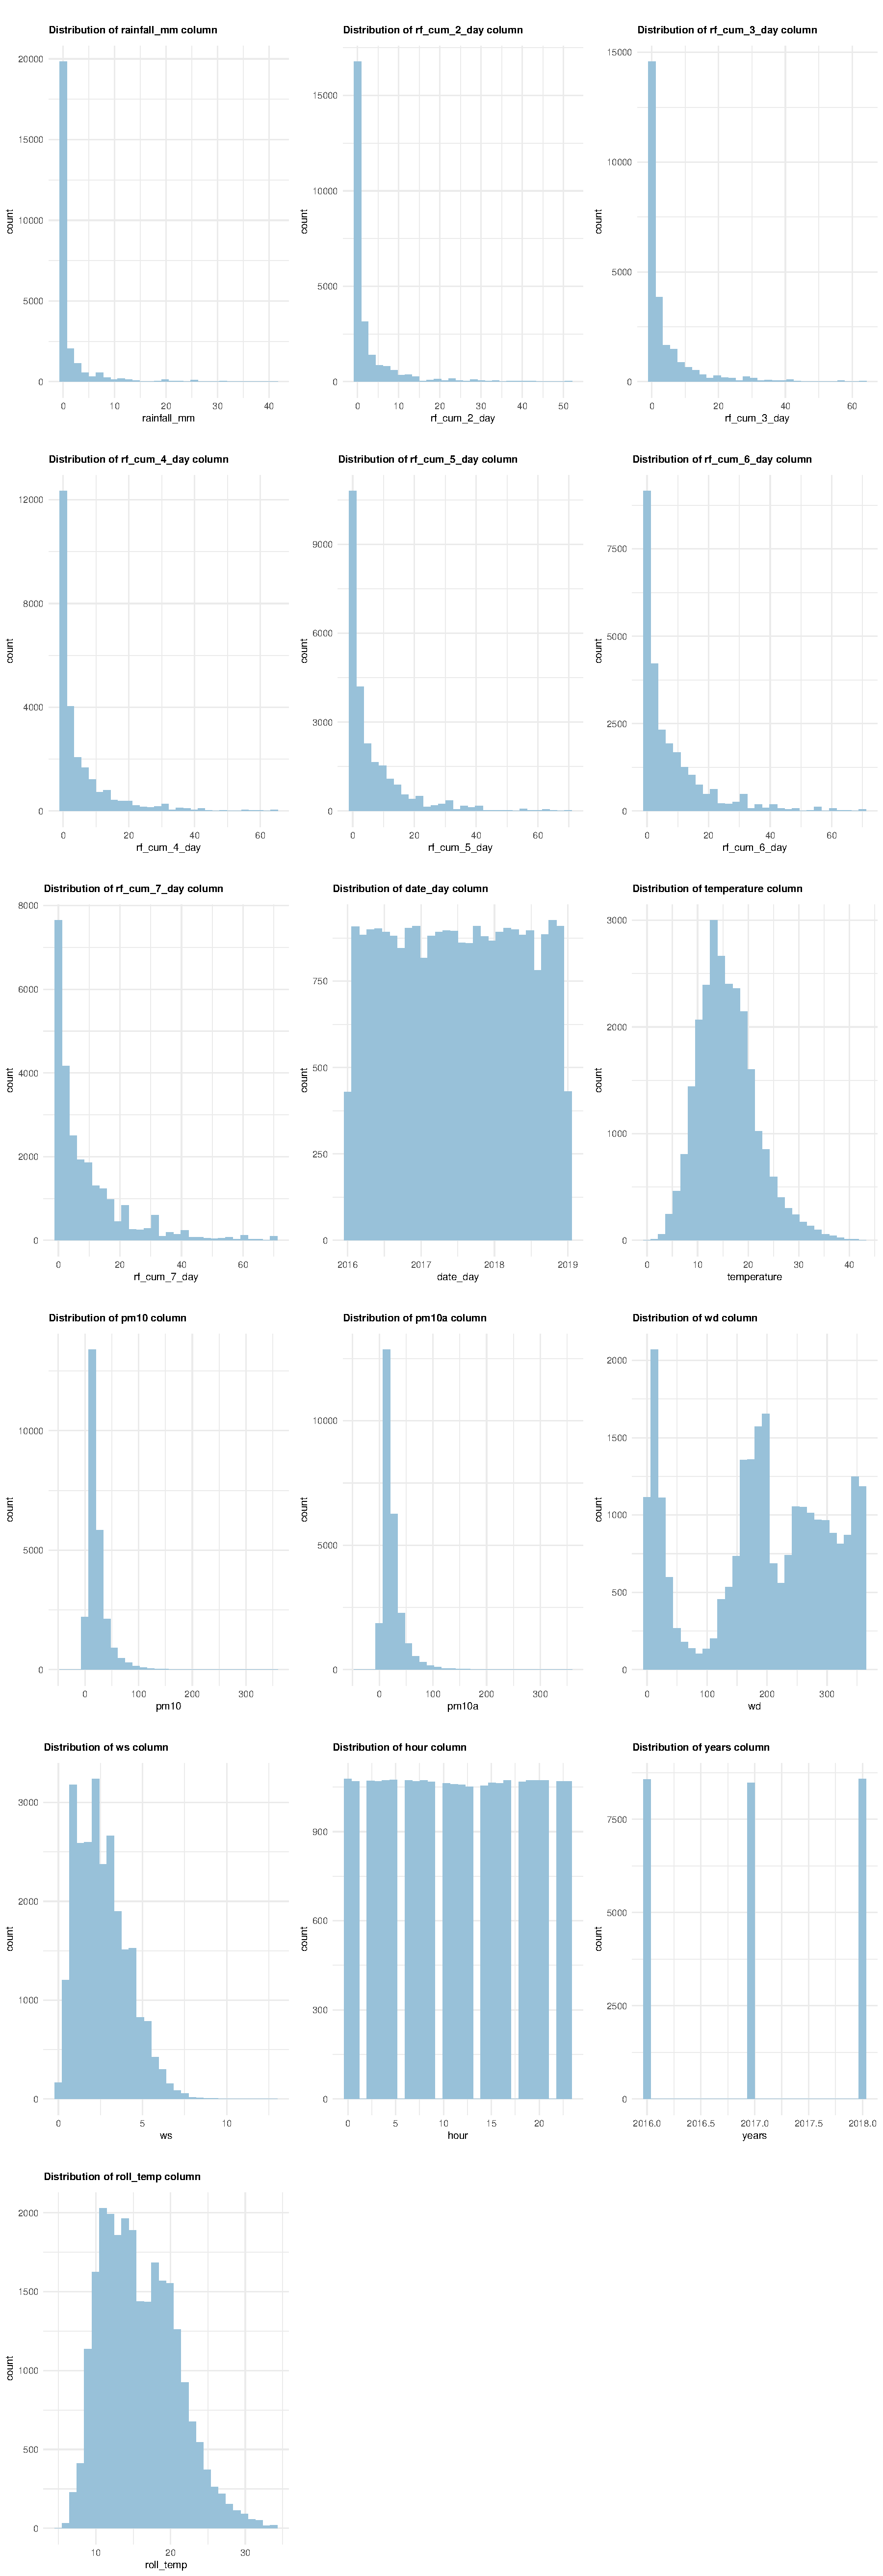
\includegraphics{MATH2269_final_project_files/figure-latex/Univariate distribution-1.pdf}
\caption{A univariate look at the distribution of all the variables
found in the Air dataset.}
\end{figure}

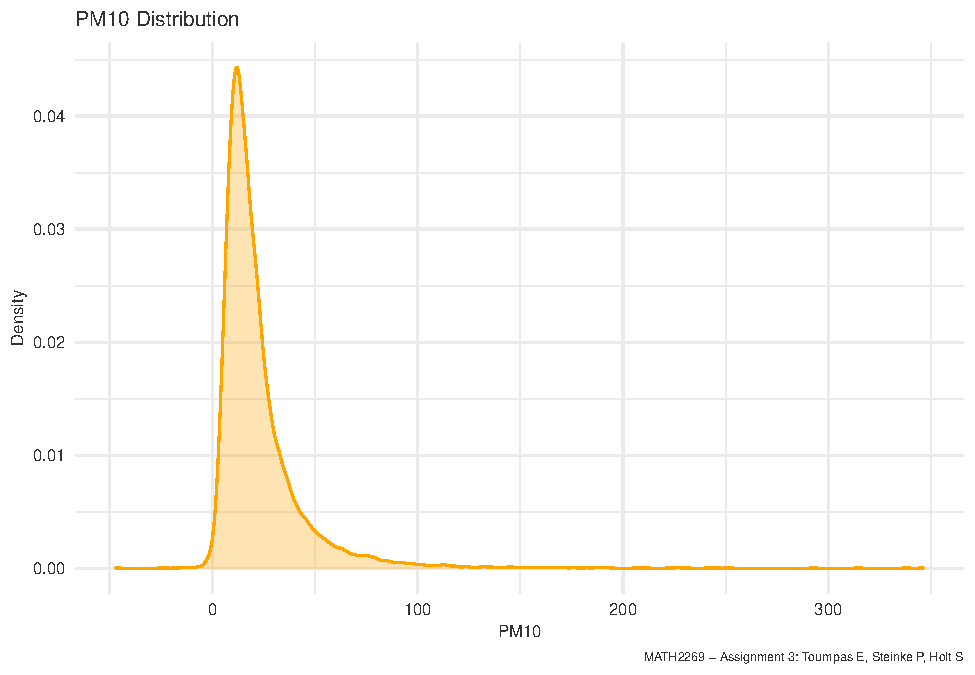
\includegraphics{MATH2269_final_project_files/figure-latex/unnamed-chunk-17-1.pdf}

\hypertarget{likelihood}{%
\subsubsection{Likelihood}\label{likelihood}}

\hypertarget{dependant-vs-independant-bivariate-visualisation}{%
\subsubsection{Dependant vs independant bivariate
visualisation}\label{dependant-vs-independant-bivariate-visualisation}}

\hypertarget{correlation-matrix-of-predictors}{%
\subsubsection{Correlation matrix of
predictors}\label{correlation-matrix-of-predictors}}

\hypertarget{subsampling}{%
\subsection{Subsampling}\label{subsampling}}

\hypertarget{subsample-size-trials}{%
\subsubsection{Subsample size trials}\label{subsample-size-trials}}

\hypertarget{subsample-selection-trials}{%
\subsubsection{Subsample selection
trials}\label{subsample-selection-trials}}

\hypertarget{mathematical-model}{%
\subsection{Mathematical model}\label{mathematical-model}}

\hypertarget{prior-specification}{%
\subsection{Prior specification}\label{prior-specification}}

\hypertarget{model}{%
\subsection{Model}\label{model}}

\hypertarget{experiments-to-improve-model-efficiency}{%
\subsection{Experiments to improve model
efficiency}\label{experiments-to-improve-model-efficiency}}

\hypertarget{isolated-experiments-on-adapt-steps}{%
\subsubsection{Isolated experiments on adapt
steps}\label{isolated-experiments-on-adapt-steps}}

\hypertarget{isolated-experiments-on-burn-in-steps}{%
\subsubsection{Isolated experiments on burn in
steps}\label{isolated-experiments-on-burn-in-steps}}

\hypertarget{isolated-experiments-on-thinning-steps}{%
\subsubsection{Isolated experiments on thinning
steps}\label{isolated-experiments-on-thinning-steps}}

\hypertarget{isolated-experiments-on-number-of-saved-steps}{%
\subsubsection{Isolated experiments on number of saved
steps}\label{isolated-experiments-on-number-of-saved-steps}}

\hypertarget{isolated-experiments-with-initial-values}{%
\subsubsection{Isolated experiments with initial
values}\label{isolated-experiments-with-initial-values}}

\hypertarget{model-fine-tuning}{%
\subsection{Model fine-tuning}\label{model-fine-tuning}}

\hypertarget{prior-sensitivity-analysis}{%
\subsection{Prior sensitivity
analysis}\label{prior-sensitivity-analysis}}

\hypertarget{posterior-inferences}{%
\subsection{Posterior Inferences}\label{posterior-inferences}}

\hypertarget{results}{%
\subsection{Results}\label{results}}

\hypertarget{prediction}{%
\subsection{Prediction}\label{prediction}}

\hypertarget{conclusion}{%
\section{Conclusion}\label{conclusion}}

\hypertarget{reference}{%
\section{Reference}\label{reference}}

\bibliographystyle{agsm}
\bibliography{bibliography.bib}

\end{document}
